\documentclass{beamer}
\setbeamertemplate{navigation symbols}{}

% there's no great way to make these "print-able"
\usetheme{Madrid}
\usecolortheme{beaver}
%\geometry{letterpaper,landscape}

% packages
\usepackage{graphicx}
\usepackage{hyperref}

% metadata
\title{Portfolio}
\author{Vaughn Kottler}
\date{\today}

% Link reference styling: blue, underlined with underline close to text
\newcommand{\HREF}[2]{{\color{blue}\underline{\smash{\href{#1}{#2}}}}}

\begin{document}

%%%%%%%%%%%%%%%%%%%%%%%%%%%%%%%%%%%%%%%%%%%%%%%%%%%%%%%%%%%%%%%%%%%%%%%%%%%%%%%
%                        Senior Design: Power Supply Module                   %
%%%%%%%%%%%%%%%%%%%%%%%%%%%%%%%%%%%%%%%%%%%%%%%%%%%%%%%%%%%%%%%%%%%%%%%%%%%%%%%

\begin{frame}
\frametitle{Senior Design: Power Supply Module}
\end{frame}

%%%%%%%%%%%%%%%%%%%%%%%%%%%%%%%%%%%%%%%%%%%%%%%%%%%%%%%%%%%%%%%%%%%%%%%%%%%%%%%
%                           Hyperloop II: Dashboard                           %
%%%%%%%%%%%%%%%%%%%%%%%%%%%%%%%%%%%%%%%%%%%%%%%%%%%%%%%%%%%%%%%%%%%%%%%%%%%%%%%

\begin{frame}
\frametitle{Hyperloop II: Dashboard}
The following slides include screenshots of the web-based dashboard I created
to monitor and control our pod for the second hyperloop competition (Summer 2017).
\break

The embedded system is one
\HREF{https://www.digikey.com/products/en/development-boards-kits-programmers/evaluation-boards-embedded-mcu-dsp/786}{STM32 Nucleo 144 F767ZI} 
microcontroller development board. We wrote all of the firmware
\HREF{https://github.com/madison-embedded/gcc-builds}{from-scratch}
and used \HREF{https://savannah.nongnu.org/projects/lwip/}{LwIP} to implement the network stack.
\break

The ``terminal'' shown in the following slides is ``redirected \texttt{stdout}'' from
the microcontroller, not an SSH session or userspace Linux program.
\break

Bootstrapping the microcontroller's serial terminal to a web-based UI is
the key feature of this UI.

\end{frame}

\begin{frame}
\frametitle{Hyperloop II: Dashboard}
    Console left (showing boot post and \texttt{help} command), data table right
\begin{center}
    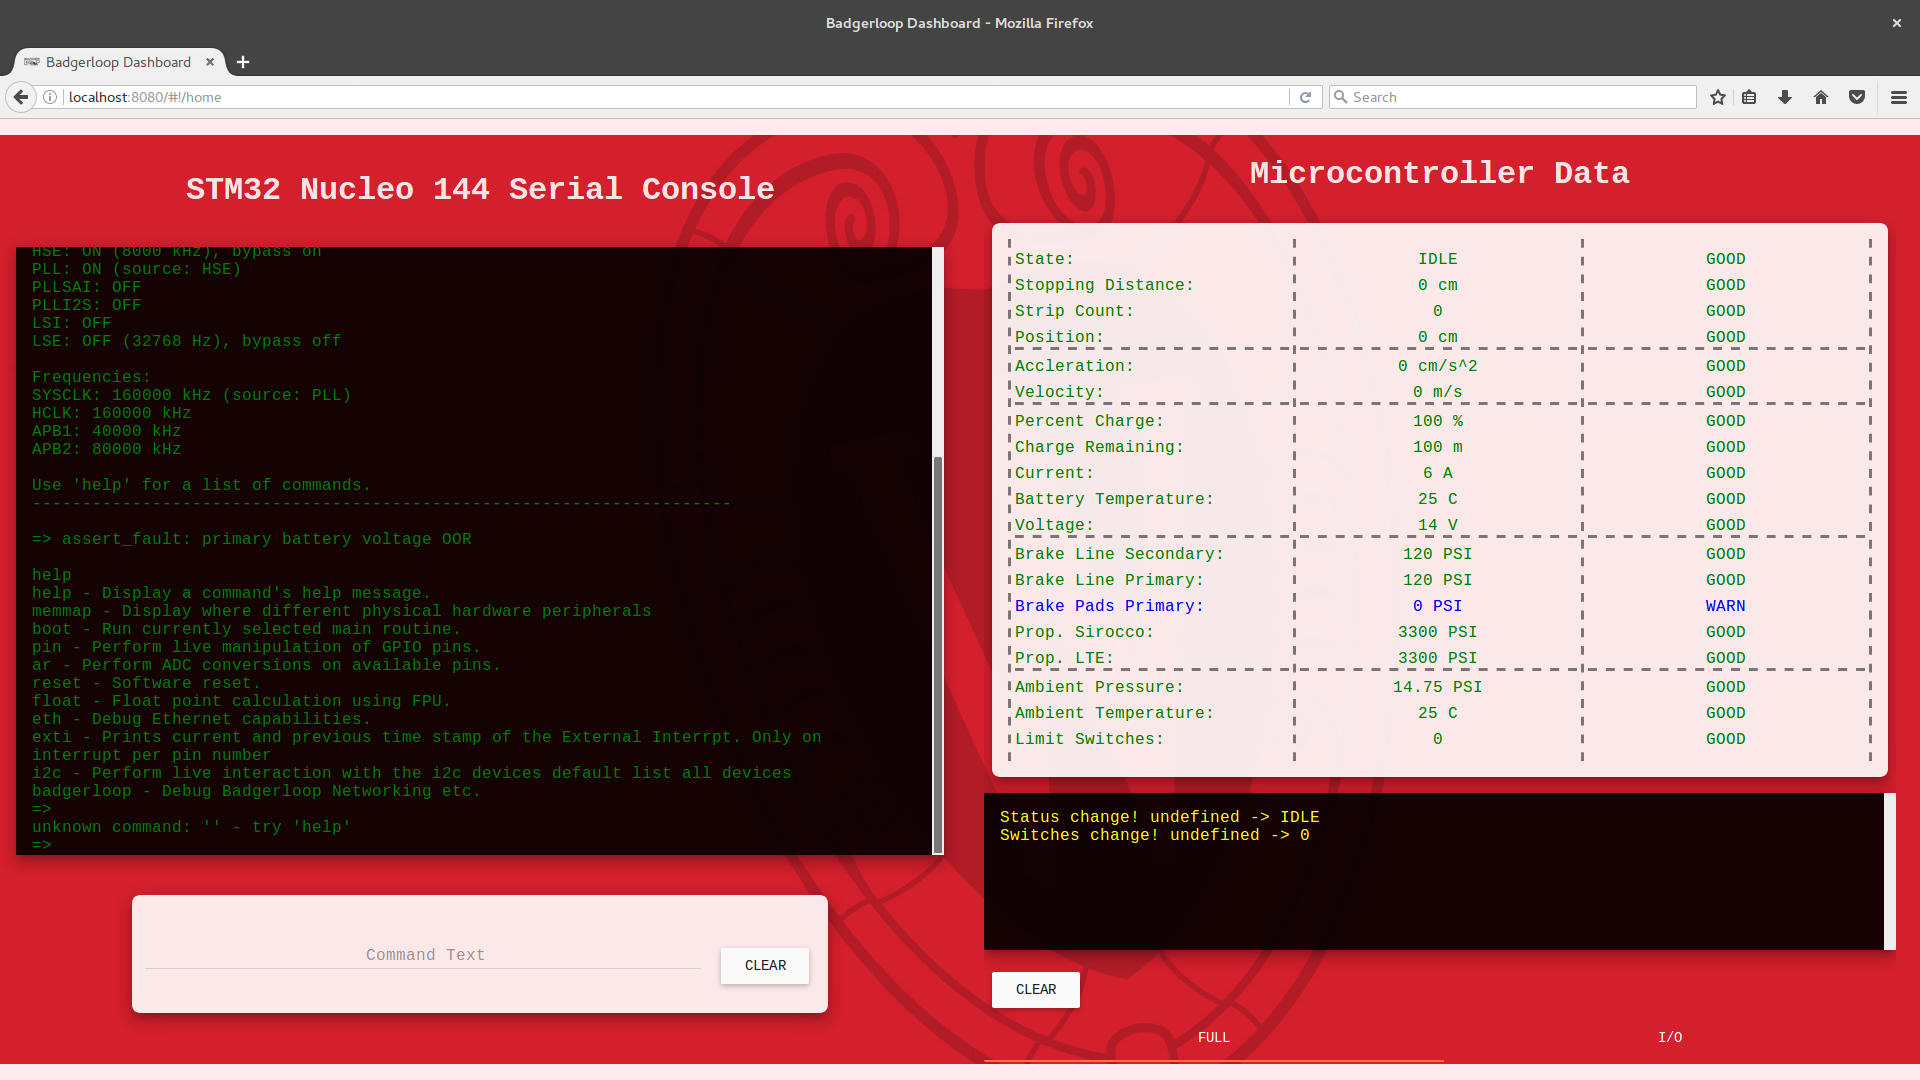
\includegraphics[width=\linewidth]{assets/badgerloop_2/Dashboard/dash_live1}
\end{center}
\end{frame}

\begin{frame}
\frametitle{Hyperloop II: Dashboard}
    Console left (showing post and \texttt{help} command), manual IO menu right
\begin{center}
    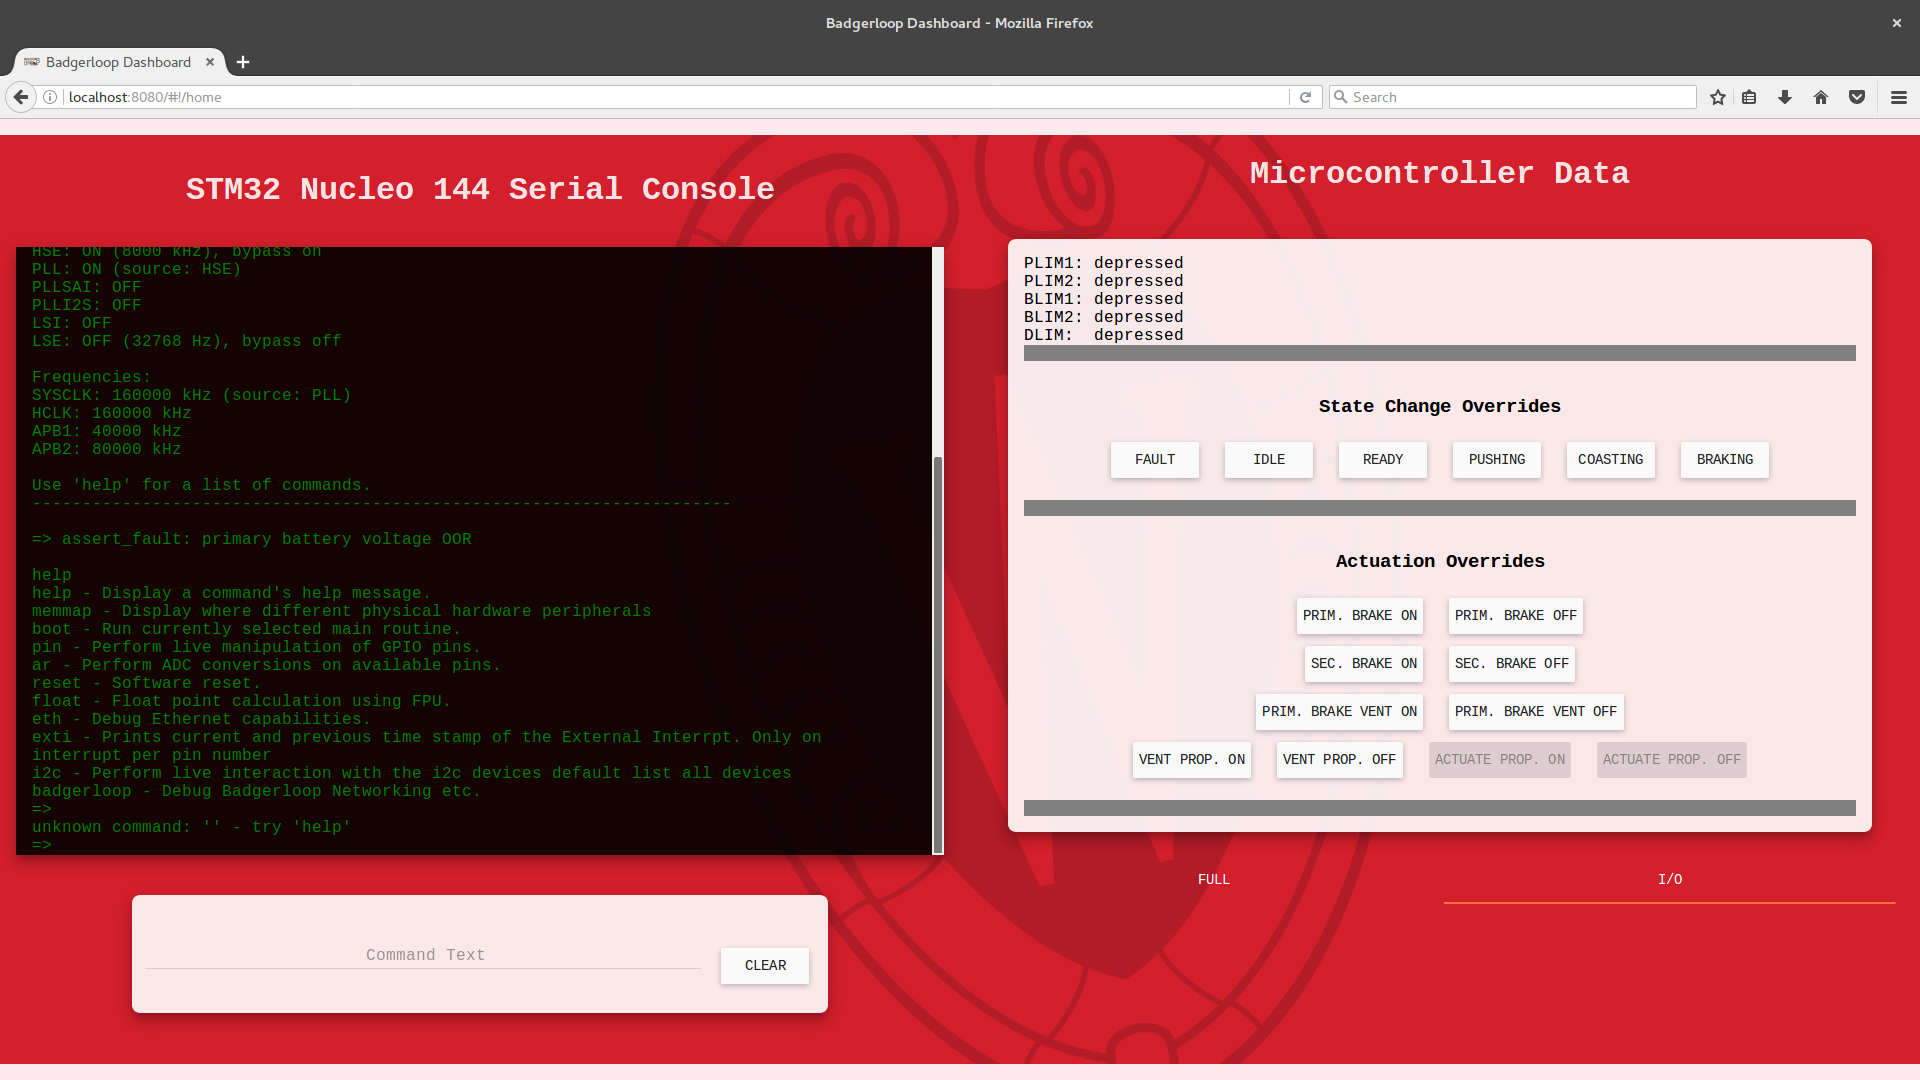
\includegraphics[width=\linewidth]{assets/badgerloop_2/Dashboard/dash_live2}
\end{center}
\end{frame}

\begin{frame}
\frametitle{Hyperloop II: Dashboard}
    \texttt{memmap} output and \texttt{badgerloop} sub-commands
\begin{center}
    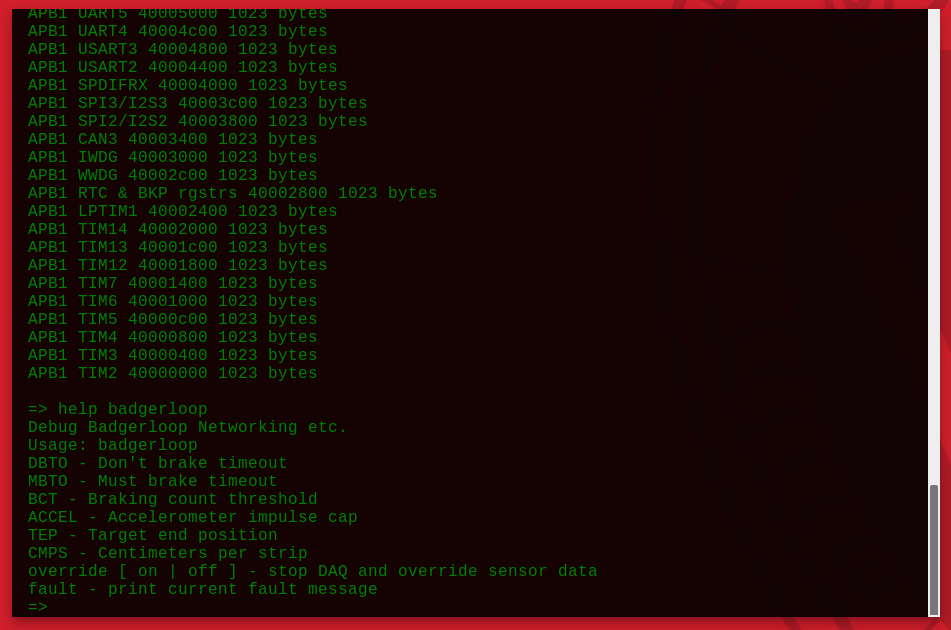
\includegraphics[width=4in]{assets/badgerloop_2/Dashboard/dash_cli_example}
\end{center}
\end{frame}

\begin{frame}
\frametitle{Hyperloop II: Dashboard}
    \texttt{ar} (analog read) command output, raw 10-bit ADC
\begin{center}
    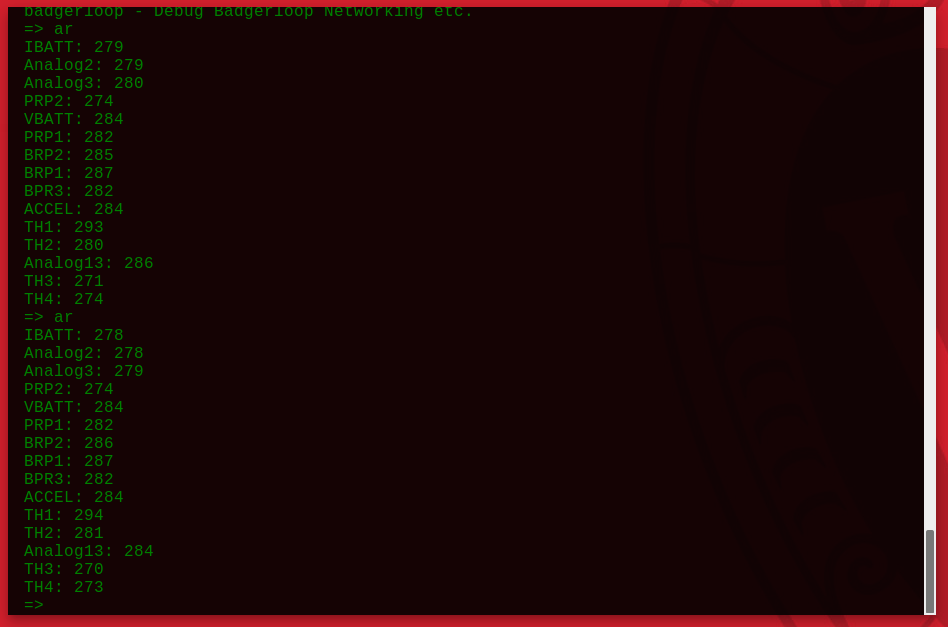
\includegraphics[width=\linewidth]{assets/badgerloop_2/Dashboard/dash_live_ar}
\end{center}
\end{frame}

\begin{frame}
\frametitle{Hyperloop II: Dashboard}
    Development on the Dashboard on the road to the competition from Wisconsin
\begin{center}
    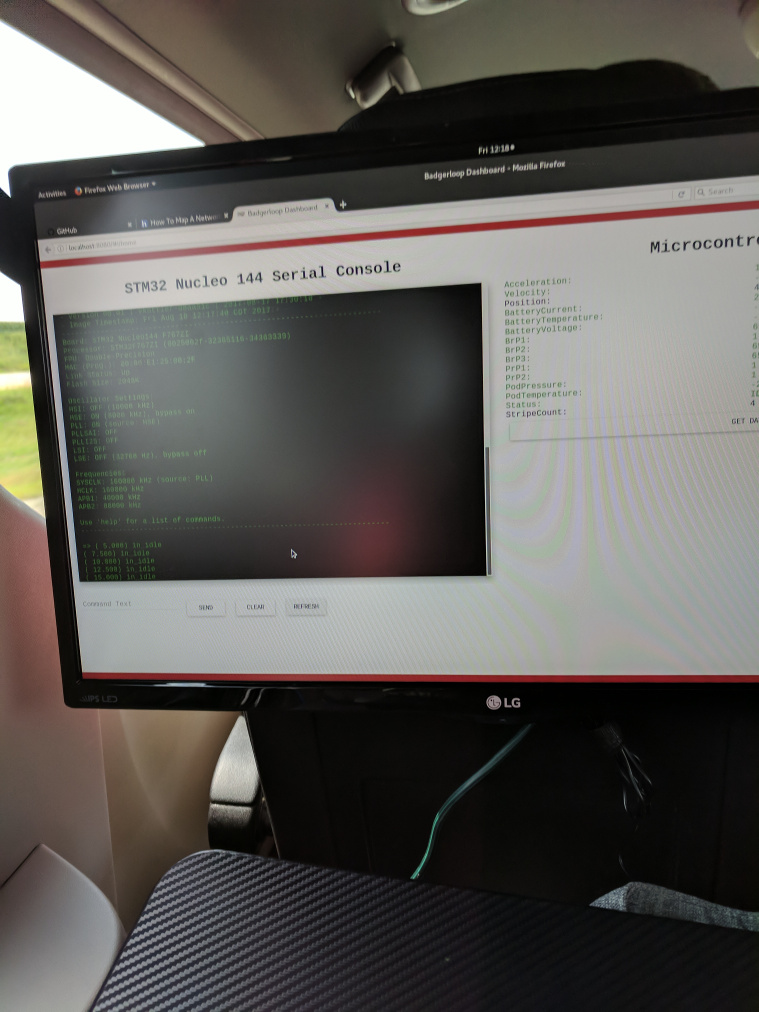
\includegraphics[height=2.5in]{assets/badgerloop_2/Dashboard/in_the_car}
\end{center}
\end{frame}

%%%%%%%%%%%%%%%%%%%%%%%%%%%%%%%%%%%%%%%%%%%%%%%%%%%%%%%%%%%%%%%%%%%%%%%%%%%%%%%

\end{document}
